\documentclass[aspectratio=169]{beamer}
\usetheme{metropolis}
\usepackage[utf8]{inputenc}
\usepackage[T1]{fontenc}
\usepackage[spanish,es-tabla]{babel}
\usepackage{amsmath,amssymb}
\usepackage{booktabs}
\usepackage{graphicx}
\usepackage{ragged2e}

\setbeamertemplate{caption}[numbered]
\setbeamertemplate{frame numbering}[fraction]
\setbeamercolor{alerted text}{fg=orange!80!black}

\newcommand{\zAI}{z_{\mathrm{AI}}}
\newcommand{\zbar}{\bar z_{\mathrm{AI}}}

\title{Artificial Intelligence in the Knowledge Economy}
\subtitle{Ide \& Talamàs (2025), \textit{Journal of Political Economy} 133(12) \\ \small Repository 5 --- Stage 1 analysis}
\author{Fabián}
\institute{AI and Economic Modeling --- Universidad del Pacífico}
\date{\today}

\begin{document}

\maketitle

% ------------------------------------------------------------
\begin{frame}{Motivación: la pregunta del paper}
\begin{block}{Pregunta}
¿Cómo reorganiza una IA \emph{escalable} la elección ocupacional, el matching entre trabajadores y expertos, y la distribución del ingreso laboral en una economía del conocimiento?
\end{block}
\vspace{0.3cm}
La respuesta depende de \alert{dos dimensiones separadas} de la tecnología:
\begin{itemize}
  \item \textbf{Autonomía}: ¿puede la IA producir por sí sola (co-worker), o solo asesorar (co-pilot)?
  \item \textbf{Capacidad} $\zAI$: ¿su conocimiento se ubica en el rango de los antiguos \emph{workers} o de los antiguos \emph{solvers}?
\end{itemize}
\vspace{0.3cm}
\footnotesize Anclas del mundo real que usa el paper: Klarna (co-worker), Harvey / GitHub Copilot (co-pilot), Agentforce; evidencia de Beane \& Anthony (2024, banca de inversión) y Litera (2022, abogados de M\&A).
\end{frame}

% ------------------------------------------------------------
\begin{frame}{Tres desarrollos que motivan el modelo (Sección 2)}
\begin{enumerate}
  \item \textbf{La IA usa conocimiento tácito a escala.} A diferencia de un humano, una vez que el conocimiento $\zAI$ está codificado, se puede copiar en tantas unidades de cómputo como se quiera.
  \item \textbf{Modelos fundacionales.} Un mismo modelo de propósito general (GPT-4, Claude, Gemini) sirve a firmas de industrias muy distintas: el conocimiento de la IA es un bien \emph{compartido}, no propietario de cada firma.
  \item \textbf{Agentes autónomos.} La IA ya no solo responde preguntas: puede iniciar y ejecutar un proyecto de principio a fin.
\end{enumerate}
\vspace{0.3cm}
\footnotesize Estas tres observaciones son las que justifican modelar $\zAI$ como fija, compartida por todas las firmas, y potencialmente autónoma.
\end{frame}

% ------------------------------------------------------------
\begin{frame}{El modelo pre-IA: jerarquías de conocimiento (Garicano)}
\begin{itemize}
  \item Masa unitaria de humanos, conocimiento $z\sim G$, densidad $g$ continua y estrictamente positiva en $[0,1]$.
  \item Cada oportunidad de producción trae un problema de dificultad $x\sim U[0,1]$.
  \item \textbf{Firma de una capa:} un productor independiente resuelve solo; output esperado $=z$.
  \item \textbf{Firma de dos capas:} un \emph{solver} $s$ atiende $n(z)$ \emph{workers} de conocimiento $z\le s$. Cada consulta cuesta $h\in(0,1)$ del tiempo del solver, la sepa resolver o no.
\end{itemize}
\begin{block}{Tamaño óptimo de equipo}
$$ n(z) = \frac{1}{h(1-z)} $$
\end{block}
\end{frame}

% ------------------------------------------------------------
\begin{frame}{Equilibrio pre-IA --- Proposición 1}
\begin{columns}
\begin{column}{0.55\textwidth}
\begin{itemize}
  \item Estratificación ocupacional: $W\preceq I\preceq S$.
  \item Matching estrictamente positivo asortativo entre workers y solvers.
  \item $I\neq\emptyset$ \emph{solo si} $h>h_0$ (para $h<h_0$ nadie produce solo).
  \item $w(z)>z$ fuera de $I$: workers y solvers ganan estrictamente más que su output en solitario --- es la prima organizacional.
\end{itemize}
\end{column}
\begin{column}{0.45\textwidth}
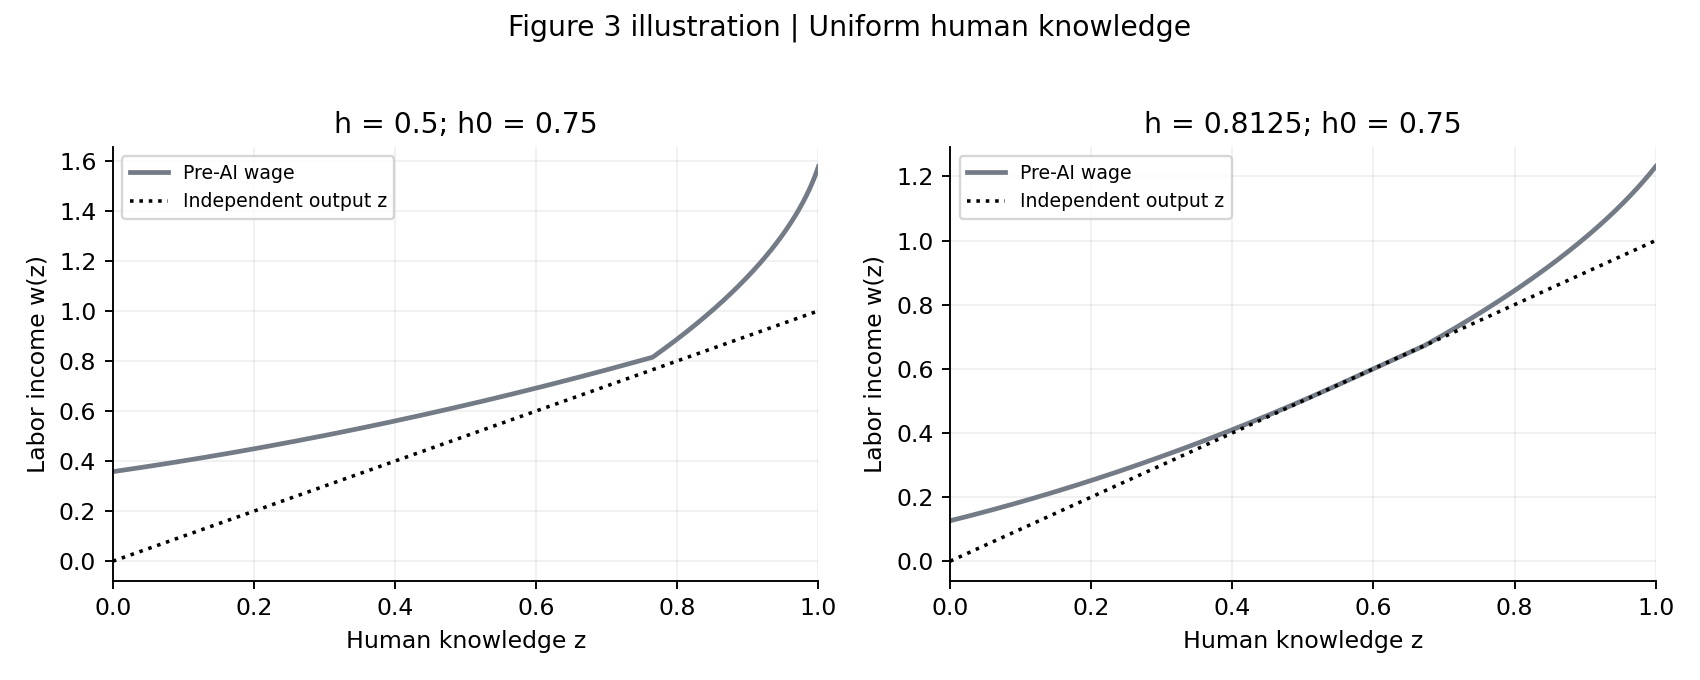
\includegraphics[width=\linewidth]{figures/fig03.png}
\end{column}
\end{columns}
\vspace{0.15cm}
{\footnotesize Reproducción propia con $G(z)=z$; panel izquierdo $h=0.5<h_0=0.75$, panel derecho $h=0.8125>h_0$.}
\end{frame}

% ------------------------------------------------------------
\begin{frame}{Modelando la IA autónoma}
\begin{itemize}
  \item La IA convierte cómputo en \textbf{agentes}, todos con el mismo conocimiento fijo $\zAI\in[0,1)$, sustitutos perfectos de un humano con ese conocimiento.
  \item \textbf{Autónoma} = puede ser \emph{co-worker} (produce) \textbf{y} \emph{co-pilot} (resuelve).
  \item El cómputo es abundante respecto al tiempo humano $\Rightarrow$ siempre sobra IA para producción independiente.
\end{itemize}
\begin{block}{Cinco configuraciones posibles de firma}
\footnotesize humano solo \quad$\vert$\quad IA sola \quad$\vert$\quad humano-solver / humanos-workers \quad$\vert$\quad IA-solver / humanos-workers \quad$\vert$\quad humano-solver / IA-workers
\end{block}
\end{frame}

% ------------------------------------------------------------
\begin{frame}{Equilibrio post-IA --- Proposición 2}
\begin{itemize}
  \item Sigue siendo único, eficiente, con estratificación y PAM: $W^*\preceq I^*\preceq S^*$, y $W^*\preceq\{\zAI\}\preceq S^*$.
  \item La IA \textbf{siempre} produce independientemente $\Rightarrow$ en equilibrio $r^*=\zAI$ y $w^*(\zAI)=\zAI$.
  \item Si $\zAI\in W$ (conocimiento de \emph{worker}), la IA necesariamente también trabaja.
  \item Si $\zAI\in S$ (conocimiento de \emph{solver}), la IA necesariamente también resuelve.
\end{itemize}
\vspace{0.2cm}
\alert{Intuición clave:} como algún cómputo queda sin pareja humana, esa fracción fija el precio $r^*$ exactamente en $\zAI$ --- el mismo mecanismo de \emph{ancla por productor independiente} que usamos más adelante en la derivación a mano.
\end{frame}

% ------------------------------------------------------------
\begin{frame}{Desplazamiento ocupacional --- Proposición 3}
\begin{columns}
\begin{column}{0.5\textwidth}
\textbf{IA básica} ($\zAI\in\mathrm{int}\,W$)
\begin{itemize}
  \item Es barata para trabajo rutinario.
  \item Los mejores solvers humanos migran a asistir a la IA.
  \item Empuja humanos marginales \emph{hacia} resolver problemas: $W^*\subset W,\ S^*\supset S$.
\end{itemize}
\end{column}
\begin{column}{0.5\textwidth}
\textbf{IA avanzada} ($\zAI\in\mathrm{int}\,S$)
\begin{itemize}
  \item Es barata para resolver problemas.
  \item Los solvers marginales migran a trabajo rutinario.
  \item Desplazamiento en la dirección \emph{opuesta}: $W^*\supset W,\ S^*\subset S$.
\end{itemize}
\end{column}
\end{columns}
\vspace{0.3cm}
\centering
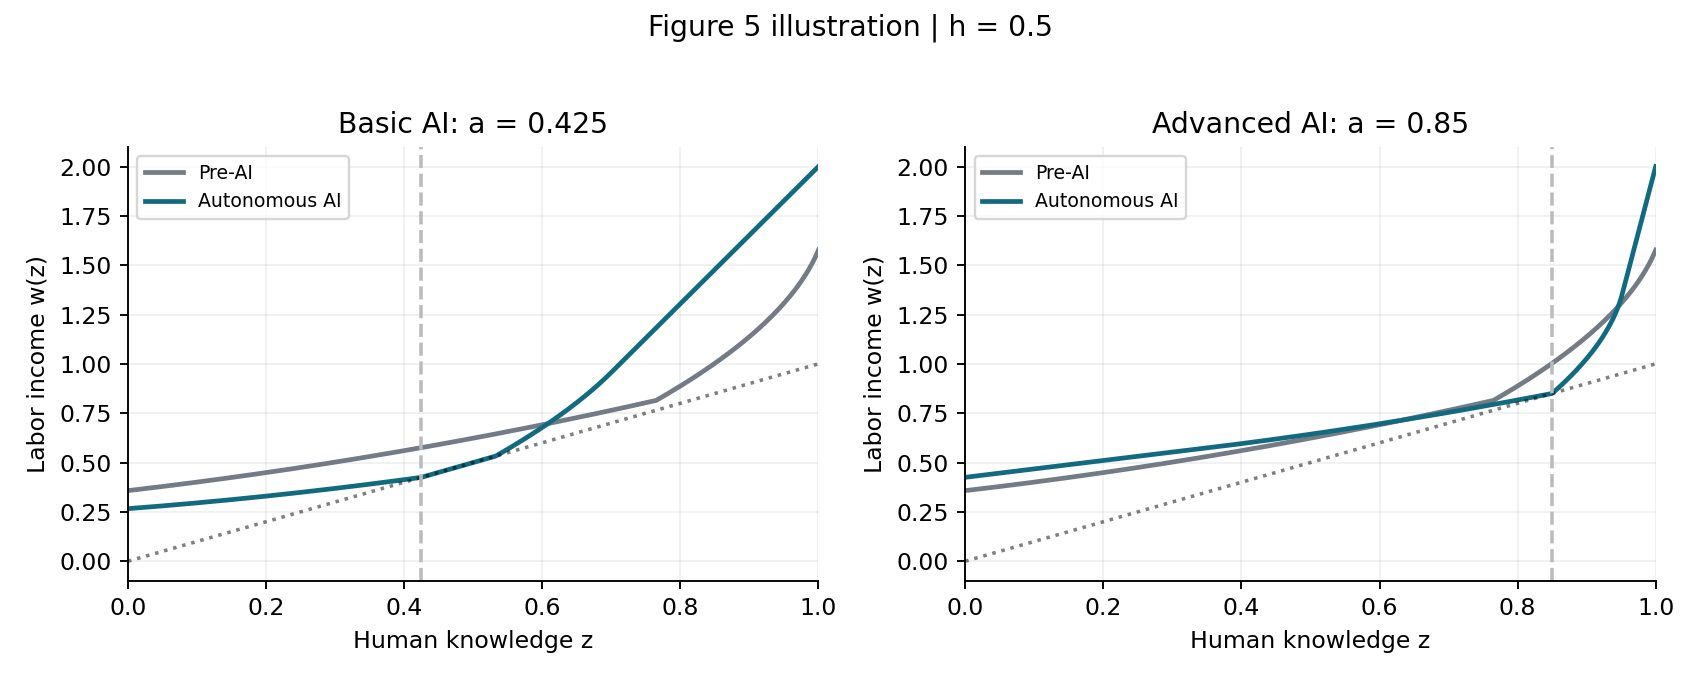
\includegraphics[height=3.6cm]{figures/fig05.png}
\end{frame}

% ------------------------------------------------------------
\begin{frame}{Productividad y \textit{span of control} --- Proposición 4}
Para quienes \textbf{no} cambian de ocupación:
\begin{itemize}
  \item Con IA básica, la productividad de los workers que siguen siendo workers \textbf{cae}: su solver humano ya no es el mejor disponible.
  \item El \textit{span of control} de los solvers que permanecen puede subir o bajar, según si su antiguo empleado era más o menos conocedor que $\zAI$.
  \item Evidencia anecdótica consistente: Litera (2022) --- abogados junior de M\&A migran a tareas complejas; Beane \& Anthony (2024) --- analistas junior de banca de inversión pierden contacto directo con socios senior.
\end{itemize}
\end{frame}

% ------------------------------------------------------------
\begin{frame}{Ingreso laboral --- Proposición 5 (el resultado central)}
\begin{itemize}
  \item El ingreso laboral total y el output \textbf{siempre suben} con la IA.
  \item Pero el individuo con $z=\zAI$ \textbf{siempre pierde} frente al pre-IA: es sustituido exactamente.
\end{itemize}
\begin{block}{Ganadores en los extremos}
Sea $B=\{z\in[0,\zAI]:w^*(z)>w(z)\}$, $T=\{z\in[\zAI,1]:w^*(z)>w(z)\}$.
$$ B\neq\emptyset \iff \zAI>\zbar,\quad \zbar\in\mathrm{int}\,W \qquad\qquad T\neq\emptyset \ \ \forall\, \zAI\in[0,1) $$
\end{block}
Los ganadores, si existen, se ubican siempre en los extremos de la distribución de conocimiento.
\end{frame}

% ------------------------------------------------------------
\begin{frame}{Descomponiendo el efecto: match vs.\ share}
Para el menos conocedor ($z=0$), la IA genera dos fuerzas opuestas:
\begin{itemize}
  \item \textbf{Efecto match (negativo):} su nuevo solver es peor que antes.
  \item \textbf{Efecto share (positivo):} el nuevo solver marginal gana solo su output en solitario (no la prima organizacional), así que el worker se queda con una porción mayor.
\end{itemize}
\centering
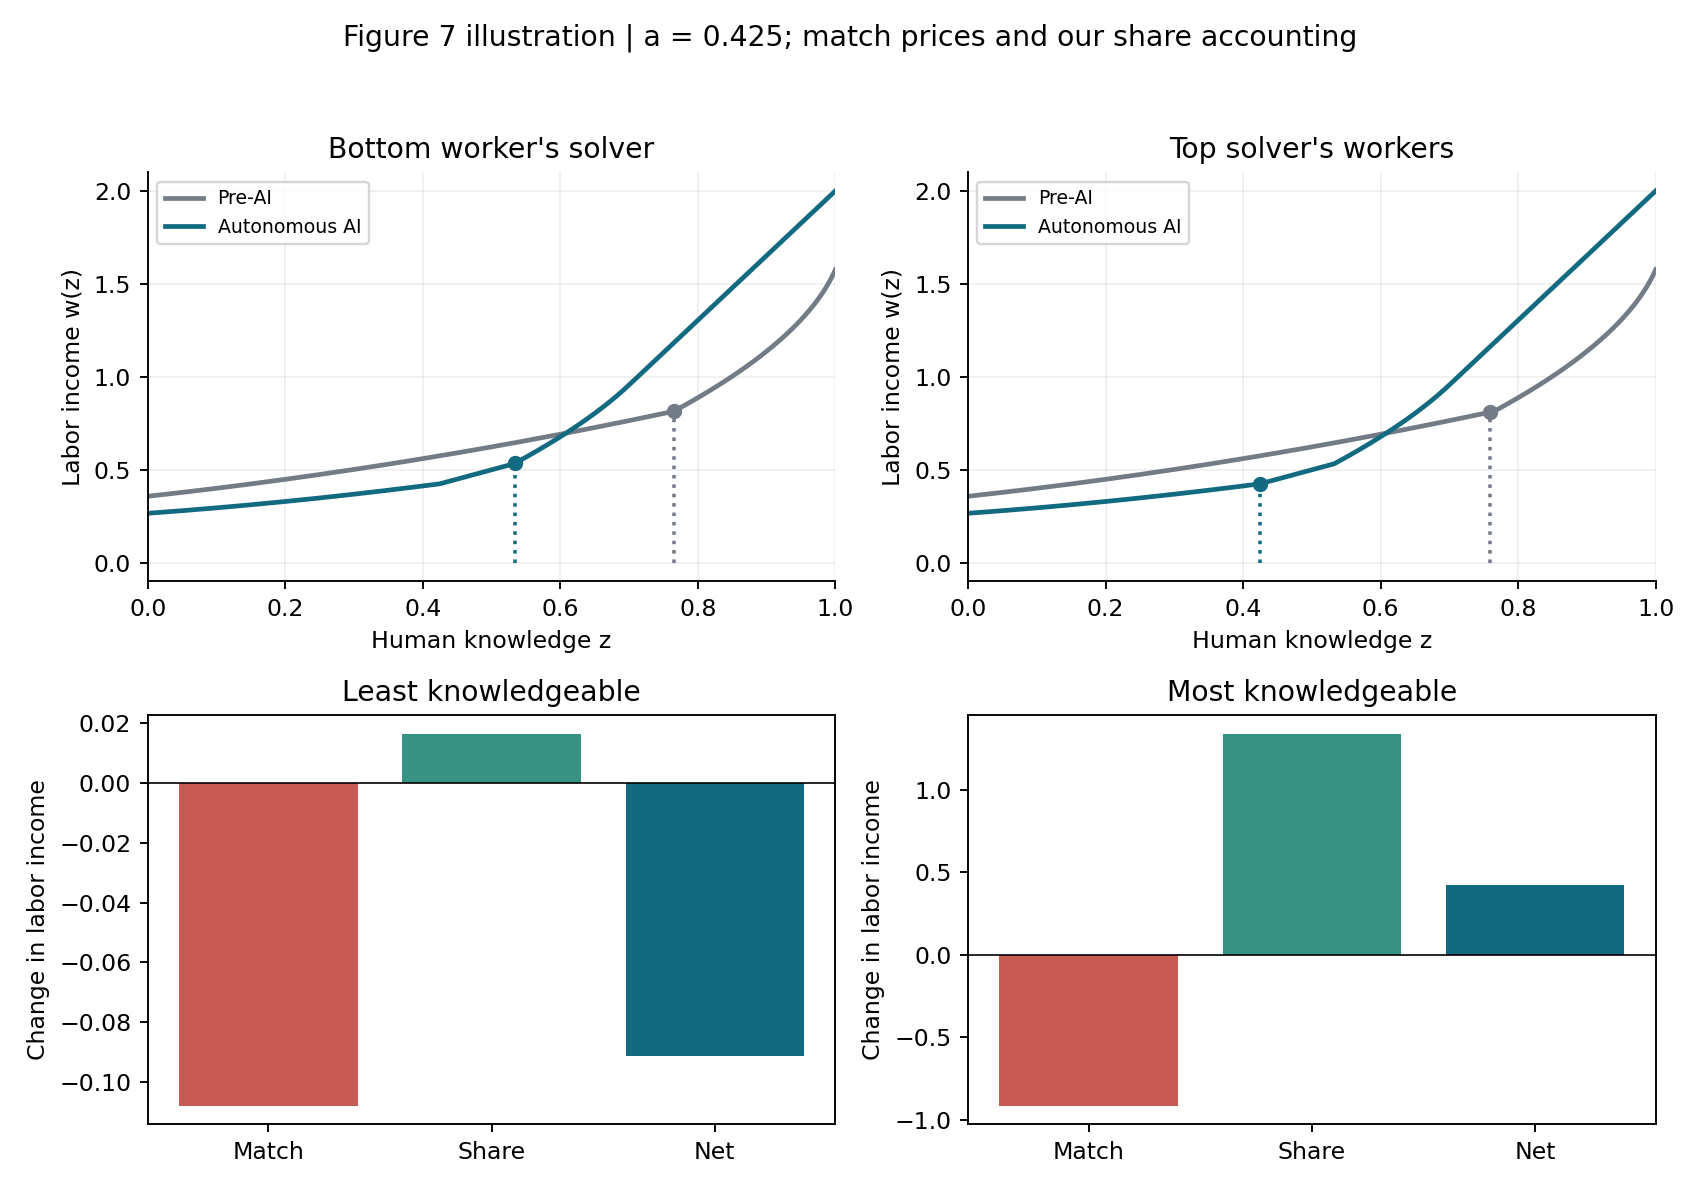
\includegraphics[width=0.85\linewidth]{figures/fig07.png}
\vspace{0.1cm}

{\footnotesize En nuestro grid ($\zAI=0.425$): abajo, match $=-0.108$, share $=+0.017$, neto $=-0.091$ (pierde). Arriba: match $=-0.915$, share $=+1.339$, neto $=+0.424$ (gana).}
\end{frame}

% ------------------------------------------------------------
\begin{frame}{La trampa: ¿autonomía o capacidad?}
\small
\begin{alertblock}{Consigna popular (incorrecta tal como se enuncia)}
\footnotesize ``El efecto distributivo lo determina la autonomía de la IA, no su capacidad.''
\end{alertblock}
\begin{itemize}\itemsep0pt
  \item $\zbar$ es un umbral de \textbf{capacidad}, definido \emph{dentro} del régimen autónomo --- la autonomía ya está fija cuando se compara.
  \item En nuestro grid: $\zbar\approx 0.715$, corte básica/avanzada $\approx 0.764$.
  \item Existe IA \textbf{básica} ($0.715<\zAI<0.764$) que \textbf{sí} beneficia a los menos conocedores --- contradice la consigna popular.
\end{itemize}
\vspace{-0.1cm}
\centering
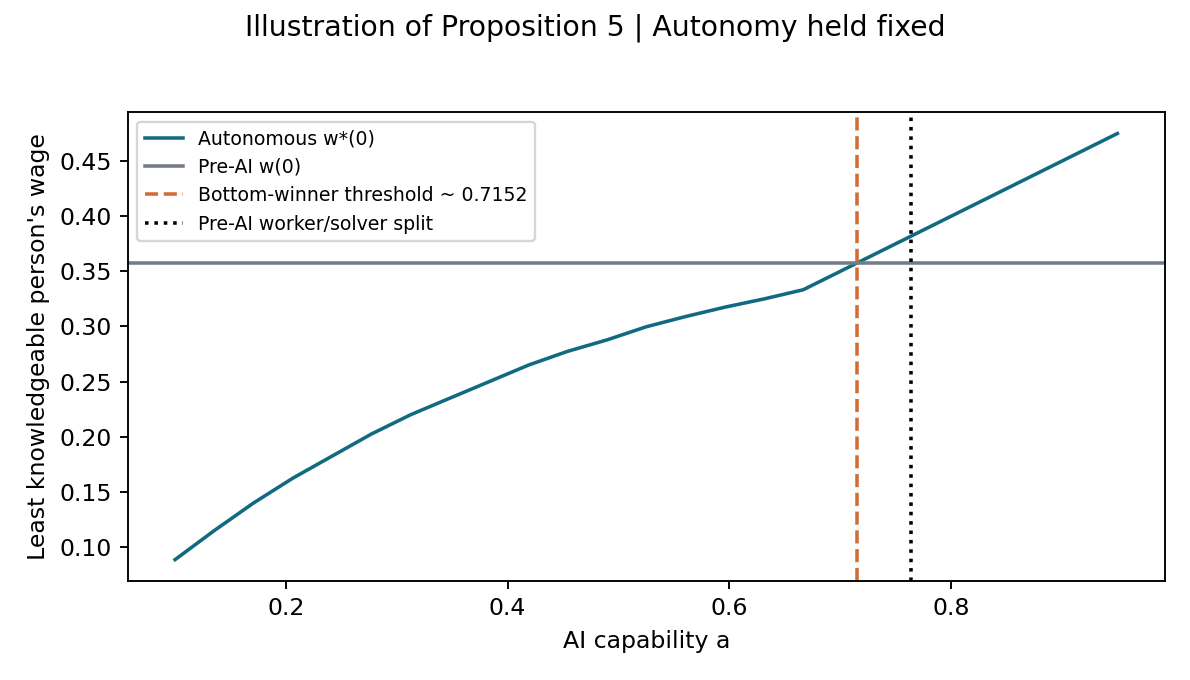
\includegraphics[width=0.52\linewidth]{figures/capability_threshold.png}
\end{frame}

% ------------------------------------------------------------
\begin{frame}{IA no autónoma --- Proposición 6}
\begin{itemize}
  \item La IA solo puede \emph{aconsejar} (co-pilot), nunca producir $\Rightarrow$ parte del cómputo queda ocioso $\Rightarrow r^\star=0$.
  \item Se adopta solo si $\zAI>w(0)$; si no, la economía es idéntica al pre-IA.
\end{itemize}
\begin{block}{Cuatro resultados, en todos los casos}
\begin{enumerate}
  \footnotesize
  \item Output estrictamente mayor con IA autónoma que no autónoma.
  \item La IA no autónoma también genera perdedores.
  \item Beneficia \textbf{más} a los menos conocedores que cualquier otro régimen (autónomo o sin IA).
  \item Beneficia \textbf{menos} a los más conocedores que la IA autónoma.
\end{enumerate}
\end{block}
\centering
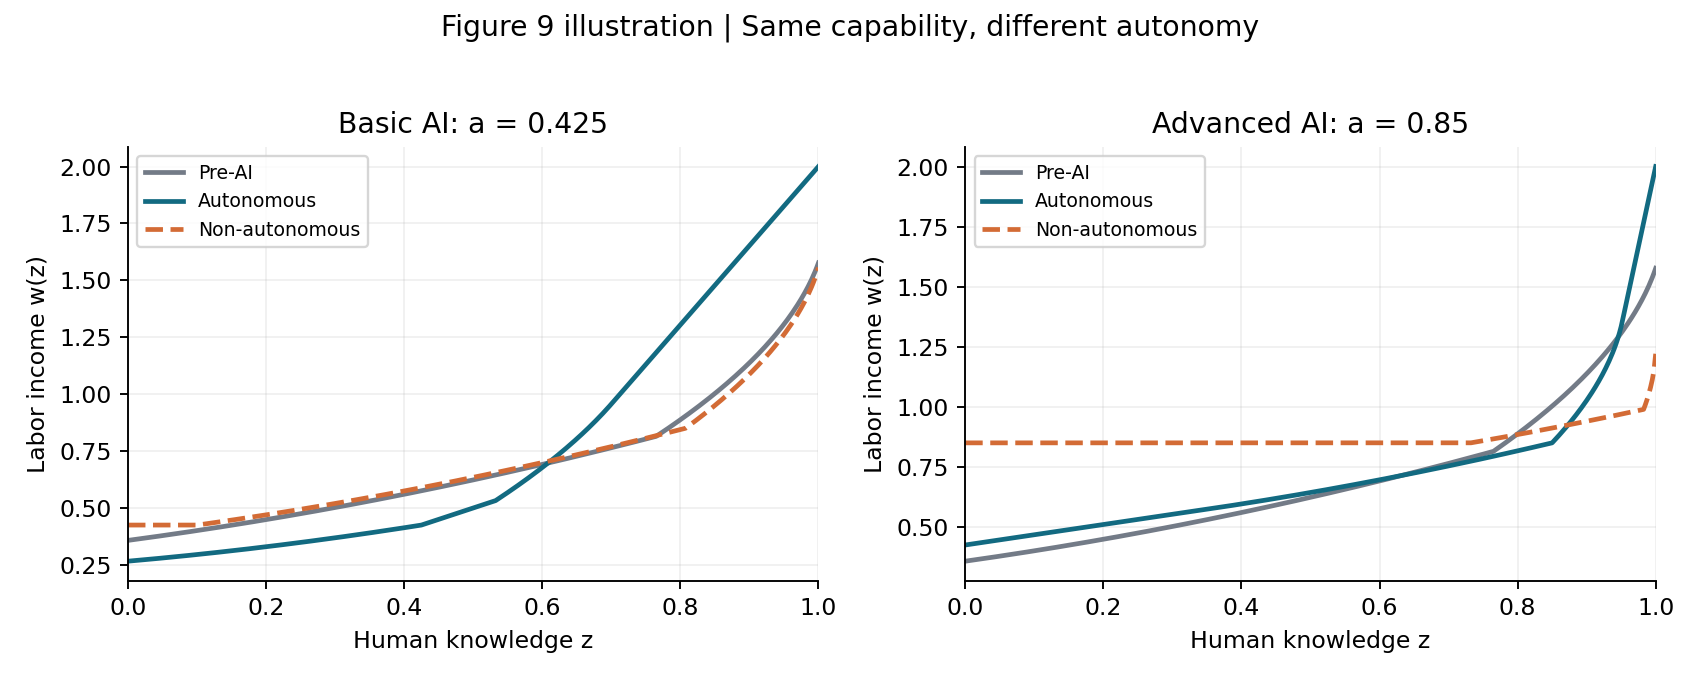
\includegraphics[height=3.3cm]{figures/fig09.png}
\end{frame}

% ------------------------------------------------------------
\begin{frame}{Resultados numéricos (nuestra reproducción, $\mu=5$)}
\centering
\begin{table}
\small
\begin{tabular}{lrr}
\toprule
Caso & Ingreso laboral & Output total \\
\midrule
Sin IA ($h=0.5$)               & 0.692 & 0.692 \\
Autónoma, $\zAI=0.425$         & 0.760 & 2.885 \\
No autónoma, $\zAI=0.425$      & 0.696 & 0.696 \\
Autónoma, $\zAI=0.85$          & 0.713 & 4.963 \\
No autónoma, $\zAI=0.85$       & 0.871 & 0.871 \\
\bottomrule
\end{tabular}
\end{table}
\vspace{0.2cm}
{\footnotesize El output autónomo alto incluye producción \emph{de la propia IA}; no debe leerse como ingreso humano. Grid de 401 tipos; con 201/801 tipos las cifras se mueven $<0.008$.}
\end{frame}

% ------------------------------------------------------------
\begin{frame}{Nuestra exploración 1: tiempo de consulta a la IA}
El paper discute (pp.\ 29--30) que un costo de tiempo para \emph{quien pregunta} es una alternativa al límite de dos capas. Lo implementamos:
$$ d(z) = 1+\tau(1-z)^2 \quad\text{tiempo por oportunidad al usar IA} $$
\begin{itemize}
  \item A $\zAI=0.85$: subir $\tau$ de 0 a 4 hace caer el salario mínimo autónomo \emph{por debajo} del nivel pre-IA.
  \item La adopción no autónoma desaparece por completo con $\tau$ alto.
\end{itemize}
\centering
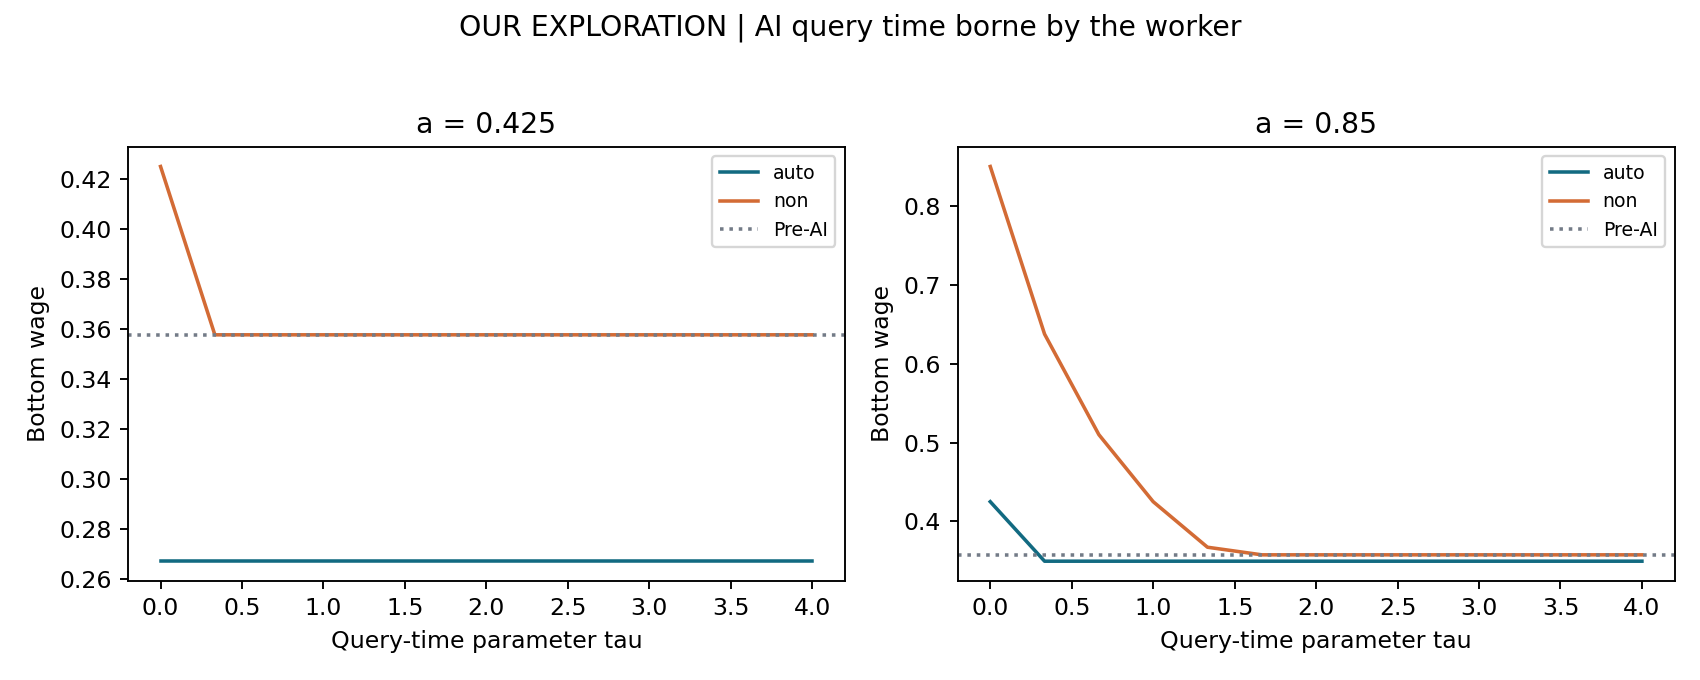
\includegraphics[width=0.8\linewidth]{figures/exploration_query_time.png}
\end{frame}

% ------------------------------------------------------------
\begin{frame}{Nuestra exploración 2: propiedad del cómputo}
Las Proposiciones 1--6 hablan de \textbf{ingreso laboral}, no de ingreso total con renta de capital.
\begin{itemize}
  \item Comparamos propiedad igualitaria del cómputo vs.\ concentrada ($\theta(z)\propto z^4$).
  \item Mismo output agregado ($\approx 2.885$) --- pero el Gini de ingreso total pasa de $\approx 0.096$ a $\approx 0.587$ con IA básica.
\end{itemize}
\centering
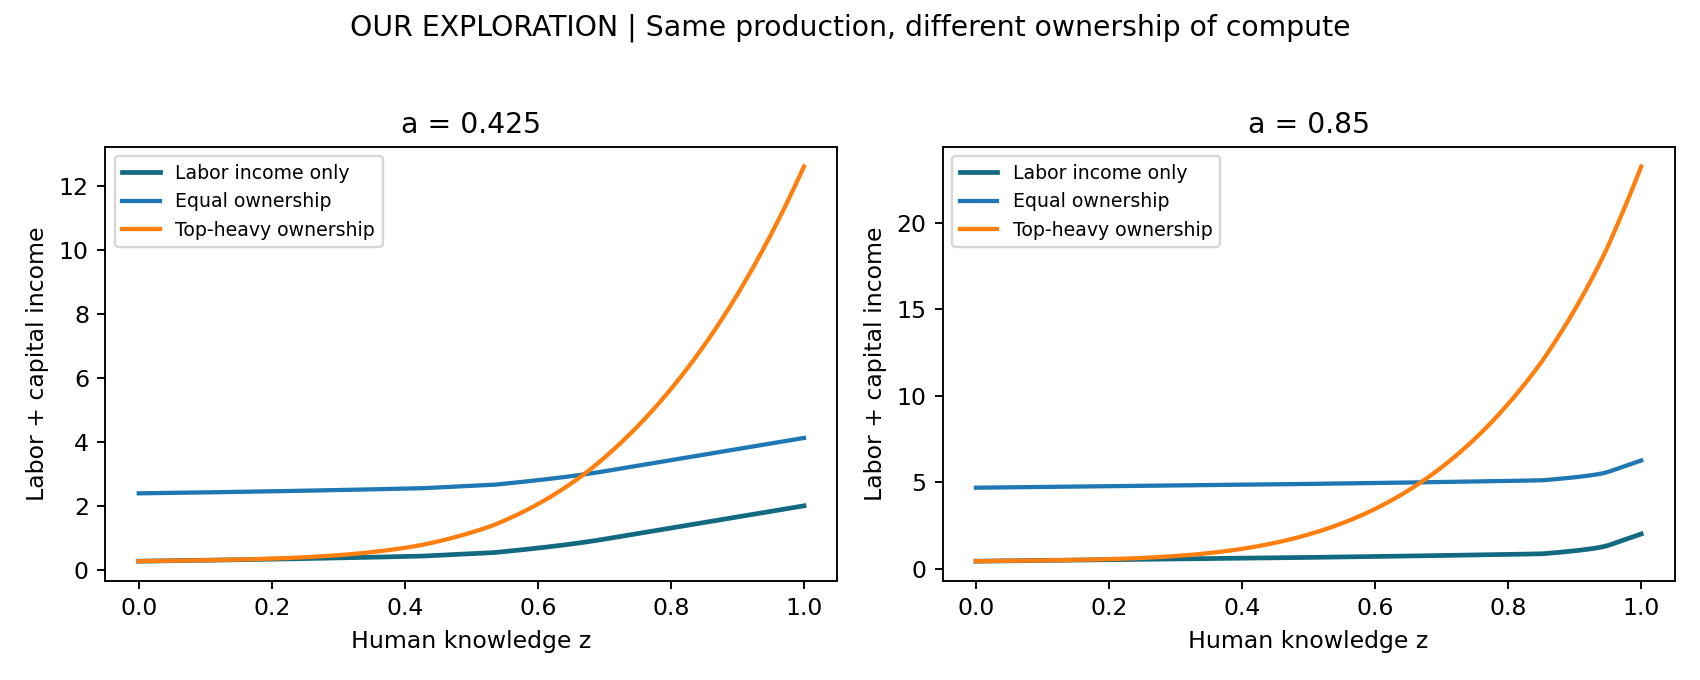
\includegraphics[width=0.8\linewidth]{figures/exploration_ownership.png}

{\footnotesize Es un ejercicio contable, no una calibración: separa el resultado del paper (salarios) del debate de política (¿quién es dueño del cómputo?).}
\end{frame}

% ------------------------------------------------------------
\begin{frame}{Derivación a mano: economía de dos tipos}
Dos tipos $z_L=0.6,\ z_H=0.9$, $h=0.5\Rightarrow n(z_L)=\dfrac{1}{h(1-z_L)}=5$.
\begin{block}{Caso 1 --- sobra capacidad de solver ($p_H=0.2,\ p_L=0.8$)}
\begin{itemize}
  \item Demanda de workers si todo $H$ resuelve: $5\times0.2=1.0>0.8$ (oferta) $\Rightarrow$ una fracción de $H$ produce sola.
  \item Esa fracción ancla $w_H=z_H=0.9$ --- el mismo mecanismo que fija $w^*(\zAI)=\zAI$ en la Proposición 2.
  \item Zero-profit: $5(0.9-w_L)-0.9=0 \Rightarrow w_L=0.72$.
  \item Cierre verificado: output $=$ ingreso laboral $=0.756$.
\end{itemize}
\end{block}
\end{frame}

% ------------------------------------------------------------
\begin{frame}{Derivación a mano: registro fotográfico (Caso 1)}
\centering
\includegraphics[height=0.82\textheight]{hand/derivacion-2tipos-caso1-p1.png}
\end{frame}

% ------------------------------------------------------------
\begin{frame}{Derivación a mano: verificación de cierre}
\centering
\includegraphics[width=0.95\linewidth]{hand/derivacion-2tipos-caso1-p2.png}
\vspace{0.4cm}
\begin{alertblock}{Alcance de esta entrega}
\footnotesize Completado: Caso 1 (sobra capacidad de solver). \textbf{Pendientes:} Caso 2 (sobra población de \textit{workers}, ancla $w_L=z_L$) y Caso 3 (balance exacto de masas), que es el que muestra que sin un tipo marginal continuo el reparto del excedente queda en un \emph{intervalo} de salarios, no en un único punto --- la pieza que conecta con por qué la Proposición 1 exige densidad continua para tener equilibrio único.
\end{alertblock}
\end{frame}

% ------------------------------------------------------------
\begin{frame}{Conclusiones e implicancias de política}
\begin{itemize}
  \item Autonomía y capacidad son dimensiones \textbf{independientes}: ninguna por sí sola determina quién gana.
  \item Existe un \textit{trade-off} output--desigualdad al regular la autonomía de la IA: la autónoma produce más, pero concentra las ganancias arriba.
  \item El marco reconcilia evidencia empírica aparentemente contradictoria: los co-pilots (Dell'Acqua et al.\ 2023, Brynjolfsson et al.\ 2025) benefician a la base; la evidencia de sustitución de trabajo de bajo conocimiento (Berger et al.\ 2024) es consistente con IA como co-worker básico.
\end{itemize}
\end{frame}

% ------------------------------------------------------------
\begin{frame}{Repositorio y referencias}
\begin{itemize}
  \item \textbf{Repo:} \texttt{github.com/fgalarzac/ai-05-ide} (rama \texttt{apoyo})
  \item \texttt{README.md} --- resumen y Proposiciones 5--6 completas
  \item \texttt{analysis.md} --- notas PAPER / DERIVATION / INTERPRETATION / OPEN QUESTION
  \item \texttt{extensions.md} --- extensiones propias vs.\ ya cubiertas por el paper
  \item \texttt{sim.py}, \texttt{figures/}, \texttt{paper/README.md} --- código, figuras, auditoría de versión
\end{itemize}
\vspace{0.4cm}
{\footnotesize Ide, E., \& Talamàs, E.\ (2025). Artificial Intelligence in the Knowledge Economy. \textit{Journal of Political Economy}, 133(12), 3762--3800. \href{https://doi.org/10.1086/737233}{DOI: 10.1086/737233}.}
\end{frame}

\end{document}
